\chapter{The workbench}
\label{ch:workbench}

The workbench is the single web page from which the whole toolbox is driven.
It holds no process state of its own: every value on the screen was read from
the HMI, the plant's fault API or the historian a moment ago. Long jobs
(dataset generation, training) run in separate processes and report progress
through files, so the page never blocks.

\section{Layout}

\begin{figure}[htbp]
\centering
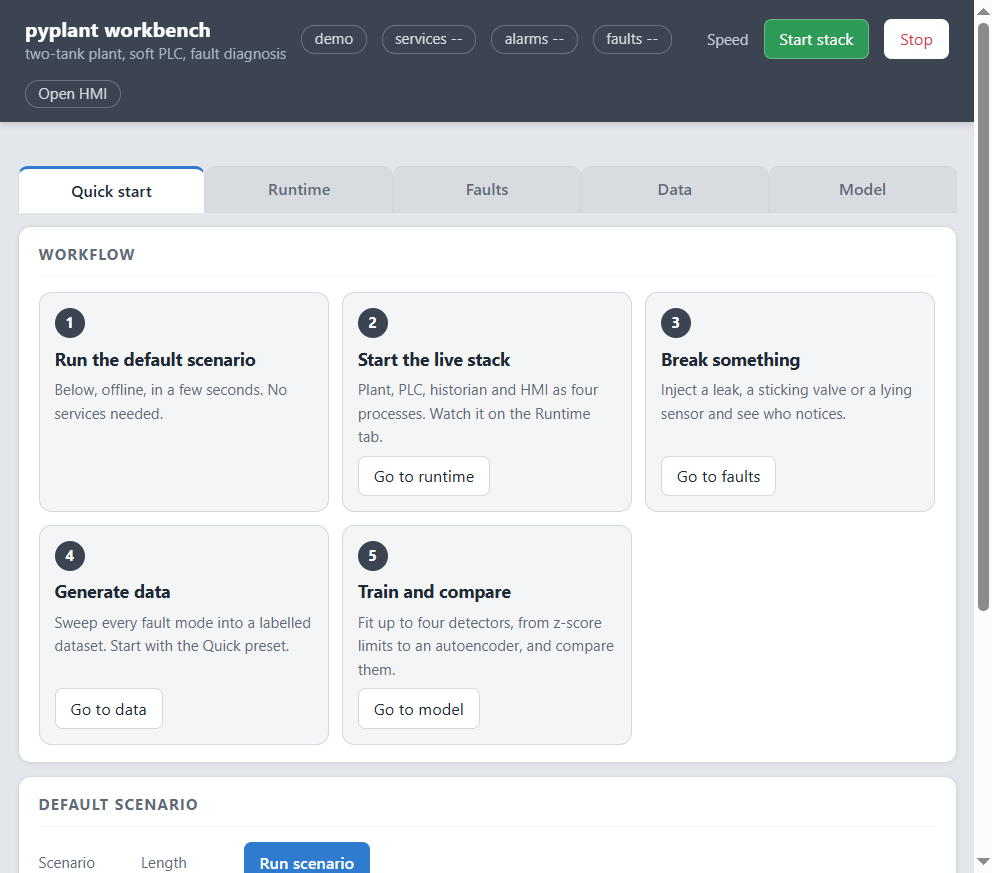
\includegraphics[width=0.6\textwidth]{quickstart_workflow.png}
\caption{The workbench header and the Quick start tab with its five workflow
cards.}
\label{fig:wb-header}
\end{figure}

\subsection*{Header}
The dark grey header stays at the top of the page and contains:
\begin{itemize}
  \item the workspace name;
  \item three status pills: services up (e.g.\ \ui{4/4 services}),
        unacknowledged alarms, and active faults. Green means healthy, amber
        partial, red attention;
  \item the \ui{Speed} selector, a real-time factor applied when the stack
        starts (Section~\ref{sec:speed});
  \item \ui{Start stack} and \ui{Stop}, which launch or terminate the four
        services in dependency order;
  \item \ui{Open HMI}, a link to the stand-alone operator page.
\end{itemize}

\subsection*{Tabs}
Below the header are five tabs. All of them are present in the page at all
times and merely hidden, so switching is instant and no callback ever fires
against a missing component.

\begin{center}
\begin{tabularx}{\textwidth}{@{}lX@{}}
\toprule
Tab & Purpose \\
\midrule
\ui{Quick start} & the opening page: workflow cards, the default scenario run offline, and a one-click live demo \\
\ui{Runtime} & service status, live mimic diagram, LIC101 faceplate and operator commands, trend, alarm list \\
\ui{Faults} & one-click fault presets, a custom fault builder, the active-fault list, ground truth against instrument readings \\
\ui{Data} & generation of the labelled scenario dataset, with presets and progress \\
\ui{Model} & selection and training of detection methods, comparison table, per-fault-mode results \\
\bottomrule
\end{tabularx}
\end{center}

\section{Quick start tab}

\subsection{Workflow cards}
Five numbered cards describe the recommended order of work. A card turns
green when its step is done, judged from what the workspace actually holds:

\begin{enumerate}
  \item \ui{Run the default scenario} --- done once a scenario has run in this session;
  \item \ui{Start the live stack} --- done while the HMI answers;
  \item \ui{Break something} --- done once any fault has been injected;
  \item \ui{Generate data} --- done once \code{dataset.parquet} exists;
  \item \ui{Train and compare} --- done once \code{artifacts/metrics.json} exists.
\end{enumerate}
Each card from step 2 on has a \ui{Go to ...} button that opens the right tab.

\subsection{Default scenario}

\begin{figure}[htbp]
\centering
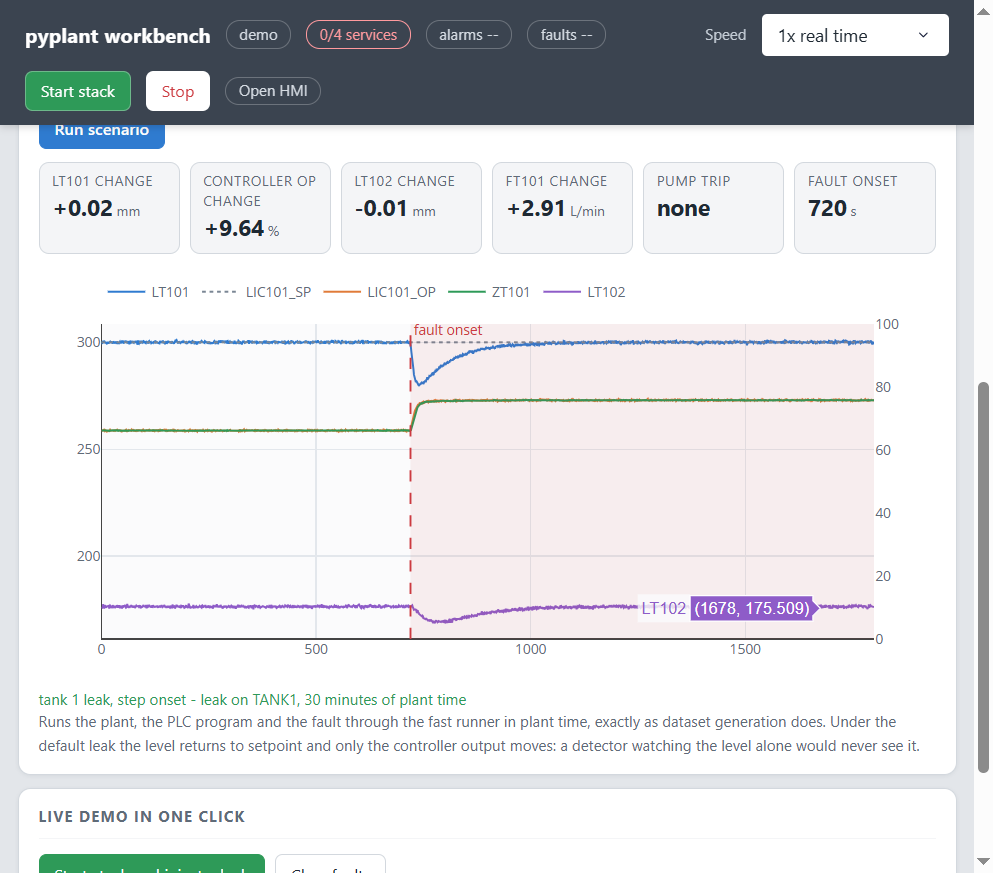
\includegraphics[width=0.6\textwidth]{quickstart_scenario.png}
\caption{The default scenario: an abrupt leak in tank 1 at $t = 720$\,s. The
level (blue) dips and returns to the setpoint (dotted); the controller output
(orange) and the valve position (green) rise by about 10\%. The summary cards
quantify the change.}
\label{fig:qs-scenario}
\end{figure}

When the page opens it immediately runs the default scenario, an abrupt leak
in tank~1, through the offline runner. No services are needed and the run
takes a few seconds. The controls are:

\begin{description}
  \item[Scenario] any of the nine library scenarios: normal operation, abrupt
        leak (default), slow leak, pump wear, fouling, valve stiction, sensor
        bias, sensor drift, frozen sensor.
  \item[Length] 15, 30 or 60 minutes of plant time. The fault starts at 40\%
        of the length.
  \item[setpoint moves] off by default, so the setpoint is held at 300\,mm and
        everything that moves is caused by the fault. Ticking it adds the
        standard setpoint programme (300, 340, 280, 300\,mm at 0, 15, 30 and
        45 minutes).
  \item[Run scenario] reruns with the chosen settings.
\end{description}

The summary cards compare the last five minutes before onset with the last
five minutes of the run: change in \tg{LT101}, controller output, \tg{LT102}
and \tg{FT101}, the time of any pump trip, and the onset time. The chart has
levels on the left axis and percentages on the right; the faulty period is
shaded red.

\subsection{Live demo in one click}
\ui{Start stack and inject a leak} starts the four services if they are not
already running, waits until each answers, and injects a
$5\times10^{-5}$\,m$^2$ leak into the live plant. Open the Runtime tab to
watch the controller output climb while the level holds. \ui{Clear faults}
removes every injected fault and leaves the instrument noise in place.

\section{Runtime tab}

\begin{description}
  \item[Services] one row per service with state, process id, port and role,
        and the exact command line the supervisor ran.
  \item[Unit 1] the mimic: pump, valve filled to its measured stem position,
        both tanks filled to their levels, flows and pump pressure. Pipes turn
        blue when they carry flow. A red frame marks a level alarm and a red
        banner a tripped interlock. Below it, cards for \tg{FT101},
        \tg{FT102}, \tg{PT101}, \tg{ZT101}, scan time and overrun count.
  \item[LIC101] the controller faceplate: PV, SP, OP, error, mode and pump
        state, plus the operator commands:
        \begin{itemize}
          \item \ui{Setpoint} + \ui{Write} --- 0 to 600\,mm. Values outside
                the span are rejected with a visible error, never clamped.
          \item \ui{Manual OP} + \ui{Write} --- valve demand in manual mode, 0 to 100\%.
          \item \ui{Auto} / \ui{Manual} --- controller mode (bumpless both ways).
          \item \ui{Start} / \ui{Stop} --- pump request.
          \item \ui{Reset interlock} --- pulses the reset bit. A latched trip
                clears only if its cause has gone.
        \end{itemize}
  \item[Trend] \tg{LT101}, \tg{LIC101_SP} and \tg{LT102} in mm on the left
        axis and \tg{LIC101_OP} in \% on the right, over 2, 5, 15 or 60
        minutes, read from the historian.
  \item[Alarms] the ISA-18.2 alarm list with priority, tag, message, state,
        time in and count, and per-row \ui{Ack} and \ui{Shelve} (30 minutes).
        \ui{Acknowledge all} acknowledges every alarm.
\end{description}

\section{Faults tab}

\begin{description}
  \item[Break something] seven presets, one click each: leak in tank 1, slow
        leak (15 minute ramp), sticking valve, worn pump, fouled interconnect,
        LT101 reading 25\,mm high, LT101 frozen. Some print a suggested next
        step; for instance a frozen transmitter on setpoint gives the
        controller nothing to act on until you move the setpoint.
  \item[Or build one] any fault kind with its own magnitude (units shown
        beside the field), sensor tag for sensor faults, and ramp time.
        Default magnitudes are filled in when the kind changes.
  \item[Active faults] id, kind, target, state, magnitude, start and ramp.
  \item[Ground truth] what each instrument reads against what the plant
        really is. Under a sensor fault the two disagree; under a process
        fault they agree and the fault appears in the controller output.
\end{description}

\begin{note}[Injection is separate from the control system]
Faults are injected through the plant's own API, not through the PLC or the
HMI. Neither the operator page nor a detector is told that a fault exists;
the only way to know is to observe the plant. This keeps the diagnosis problem
honest.
\end{note}

\section{Data tab}

\begin{description}
  \item[Preset] fills the four fields below:
  \begin{center}
  \begin{tabular}{@{}lrrrrr@{}}
  \toprule
  Preset & Run length & Magnitudes & Repeats & Normal runs & Typical time \\
  \midrule
  Quick & 1200\,s & 1 & 1 & 6 & about 1.5 min \\
  Standard & 3600\,s & 3 & 2 & 10 & about 4 min \\
  Thorough & 3600\,s & 5 & 3 & 16 & about 10 min \\
  \bottomrule
  \end{tabular}
  \end{center}
  \item[Run length] seconds of recorded plant time per run.
  \item[Magnitudes] how many fault sizes per mode, spread from 0.5 to 1.5
        times the library value.
  \item[Repeats] runs per mode and magnitude, each with its own seed and a
        random onset between 25\% and 60\% of the run.
  \item[Normal runs] fault-free runs. At least three are needed (train,
        calibrate, test); more give a better false-alarm estimate.
  \item[Generate / Cancel] start or stop the background job. The progress bar
        and \ui{Recent runs} table update every three seconds.
\end{description}

\section{Model tab}

\begin{figure}[htbp]
\centering
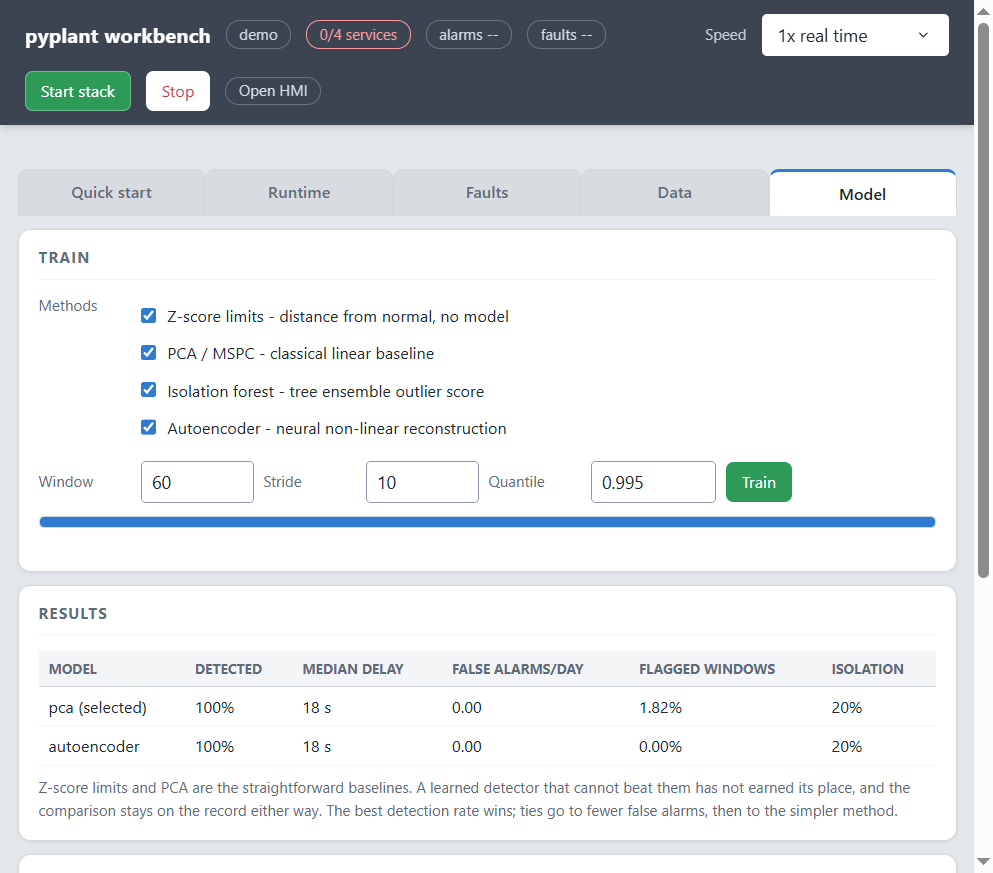
\includegraphics[width=0.6\textwidth]{model_tab.png}
\caption{The Model tab: method selection, window settings and the comparison
table.}
\label{fig:model-tab}
\end{figure}

\begin{description}
  \item[Methods] tick any of the four detectors (Chapter~\ref{ch:ml} and
        \ref{ch:dl}): z-score limits, PCA/MSPC, isolation forest, autoencoder.
  \item[Window] samples per window (1\,Hz, so 60 is one minute).
  \item[Stride] samples between consecutive windows.
  \item[Quantile] the fraction of held-out normal windows that must lie below
        the alarm threshold, e.g.\ 0.995.
  \item[Train] fits every ticked method, evaluates it and deploys the best.
  \item[Results] detection rate, median detection delay, false alarms per
        day, flagged-window rate and isolation accuracy per method.
  \item[By fault mode] for the selected method: runs, detection rate, median
        delay, the channel that contributed most, and the channel physics
        expects.
\end{description}

\section{Speed}
\label{sec:speed}

Speed is a real-time factor applied to both the plant and the PLC tickers:
at $4\times$ a 100\,ms scan runs every 25\,ms of wall time. Slow faults need
it: a stiction limit cycle takes several process time constants to establish,
and this plant's time constant is 72\,s.

\begin{warn}[Windows timer granularity]
Windows schedules sleeps in steps of about 15.6\,ms. Above $4\times$ the scan
period falls below that, every scan lands late and \tg{SCAN_OVERRUNS} climbs.
The controller still works; the diagnostics are telling the truth. Keep speed
at 4 or below on Windows. Linux and macOS manage $20\times$.
\end{warn}
